\documentclass[UTF8]{ctexbook}
\usepackage{graphicx}
\usepackage{amsmath}

\title{桥梁大作业报告}
\author{组长:贺琪 \\ 组员:陈煜 \ 刘畅武 \ 杨昊光 \ 朱子霖}

\begin{document}
\maketitle

\tableofcontents

%-------------------------这里是这个项目的整体描述---------------------------------
%----------------------------------------------------------------------------------
\newpage
\section{总述}
\subsection{项目描述}
桥模型由桥墩(pier),桥面(floor),支撑梁(support beam),河堤(river bank)和钢缆(cables)五部分组成,其中桥墩和河堤用实体单元建模,桥面用板单元建模,支撑梁用梁单元建模,钢缆用杆单元建模,如图1 所示。\\
\begin{center}
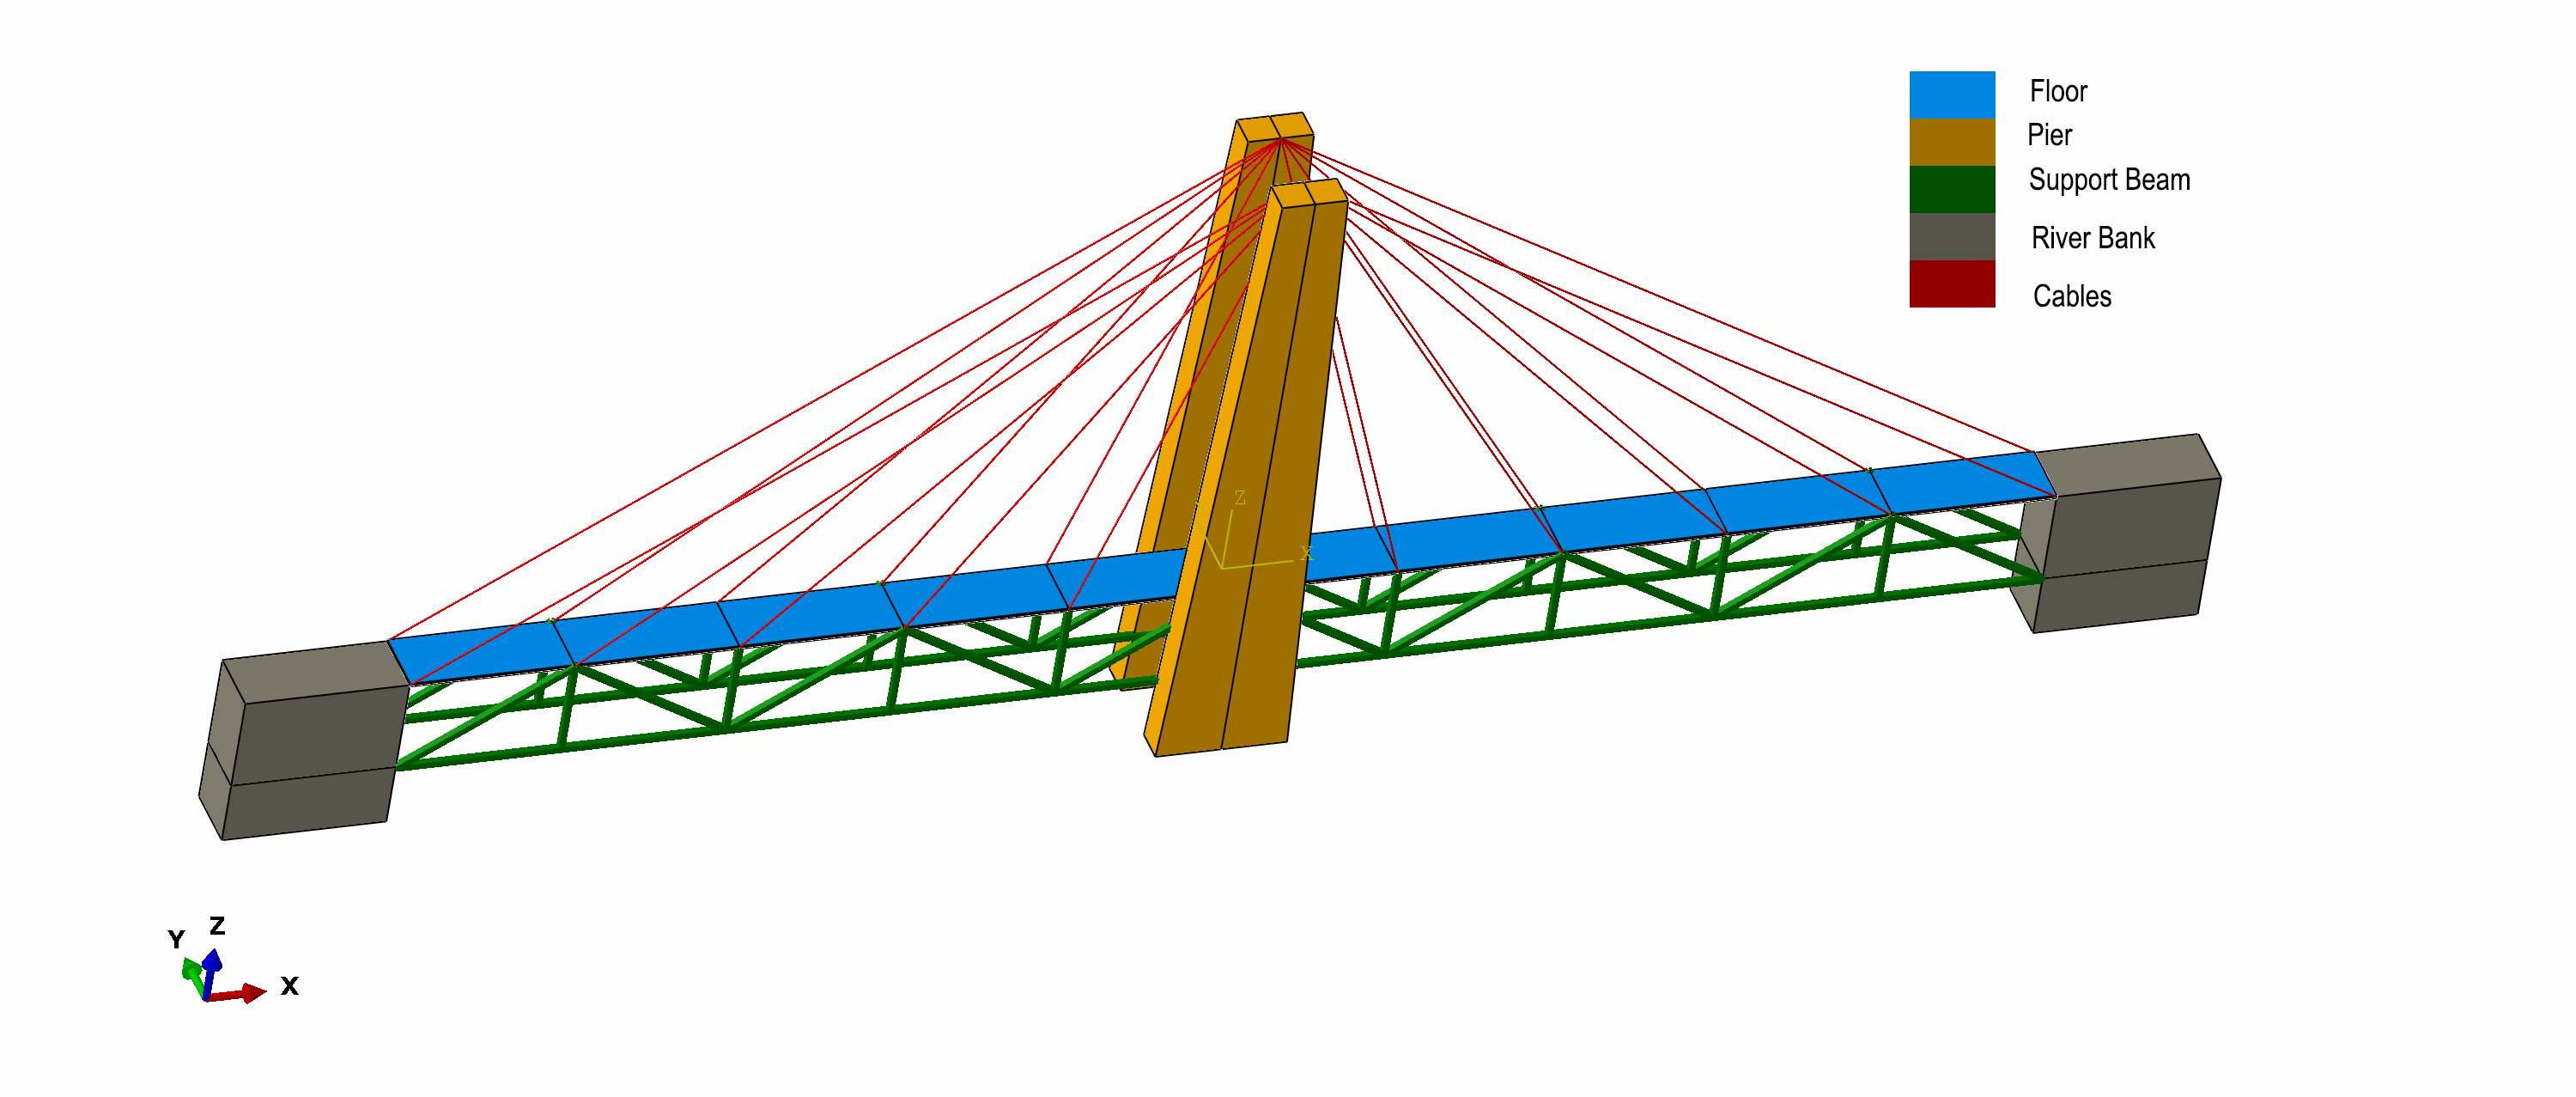
\includegraphics[width=0.6\textwidth]{01.png} % Include the image placeholder.png
\end{center}

\textbf{桥墩}:

桥墩在XZ方向为左右对称梯形,如图2所示,梯形高200,上底为20,下底40,在y方向上厚度为10。桥面位于距桥墩底50处。两个桥墩顶面内侧中点为所有钢缆的与桥墩的连接点。(参照图1)

采用实体单元建模

\begin{center}
\begin{tabular}{ll}
材料&:Concrete\\
弹性模量&:25e9\\
泊松比&:0.3\\
密度&:2320\\
\end{tabular}
\end{center}

\begin{center}
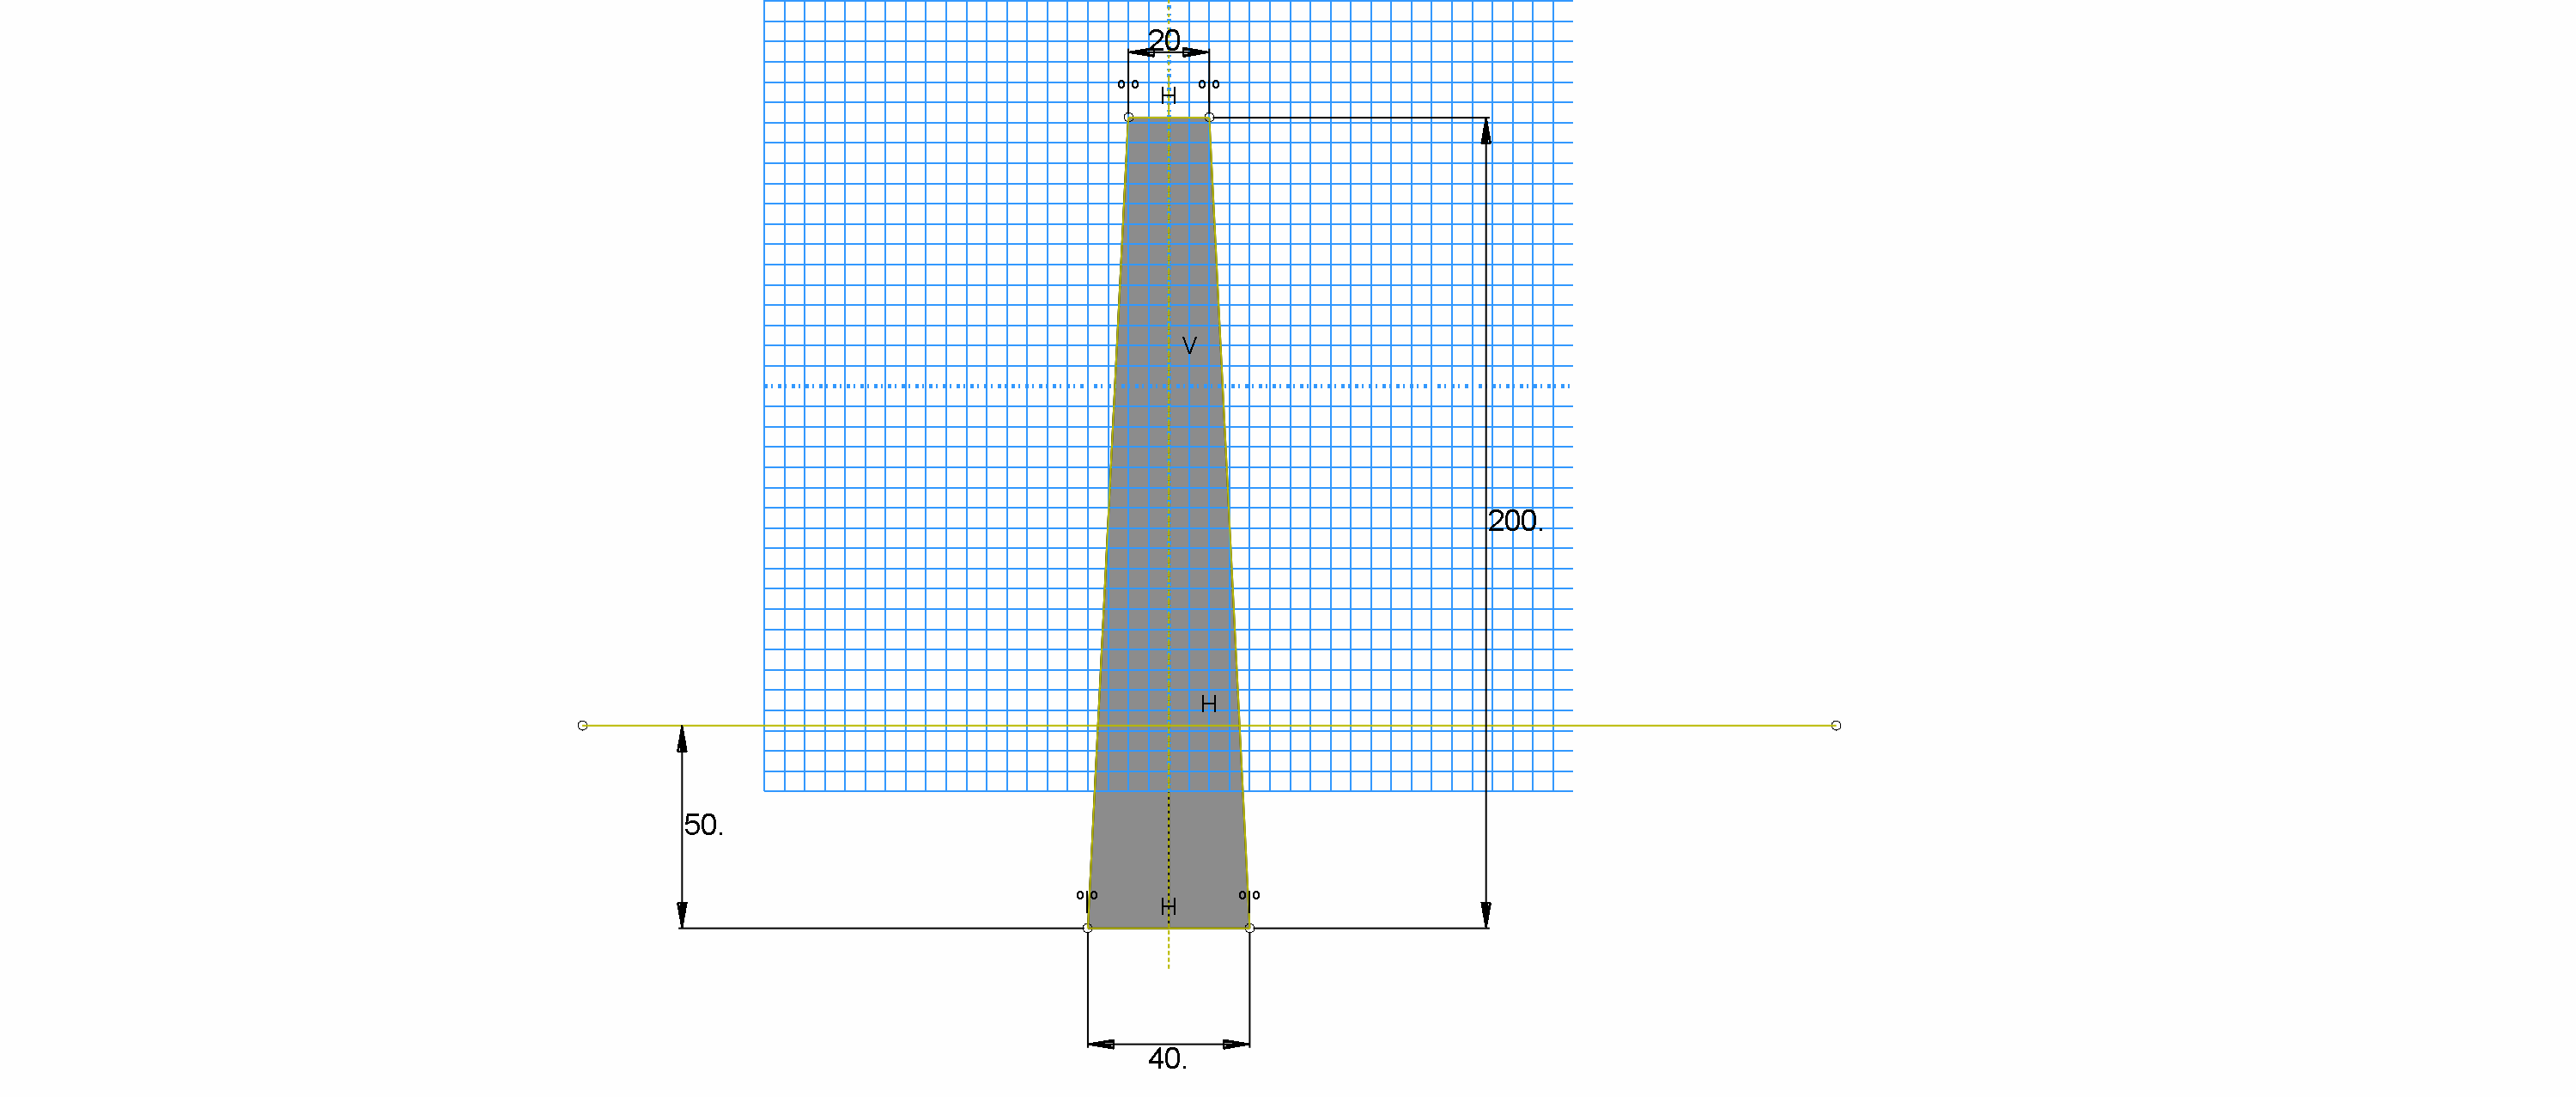
\includegraphics[width=0.6\textwidth]{02.png}
\end{center}

\textbf{桥面}:

桥面位于z=0的平面内,如图3所示,为长方形,长为500,宽为20,厚度为1。在桥面上下边对称地布置钢缆连接点,每个钢缆连接点相距50,共计2×2×5=20个钢缆连接点。每根钢缆另一端连接桥墩顶面内侧中点。(参照图1)

采用板单元建模

\begin{center}
\begin{tabular}{ll}
材料&:Concrete\\
弹性模量&:25e9\\
泊松比&:0.3\\
密度&:2320\\
\end{tabular}
\end{center}
\begin{center}
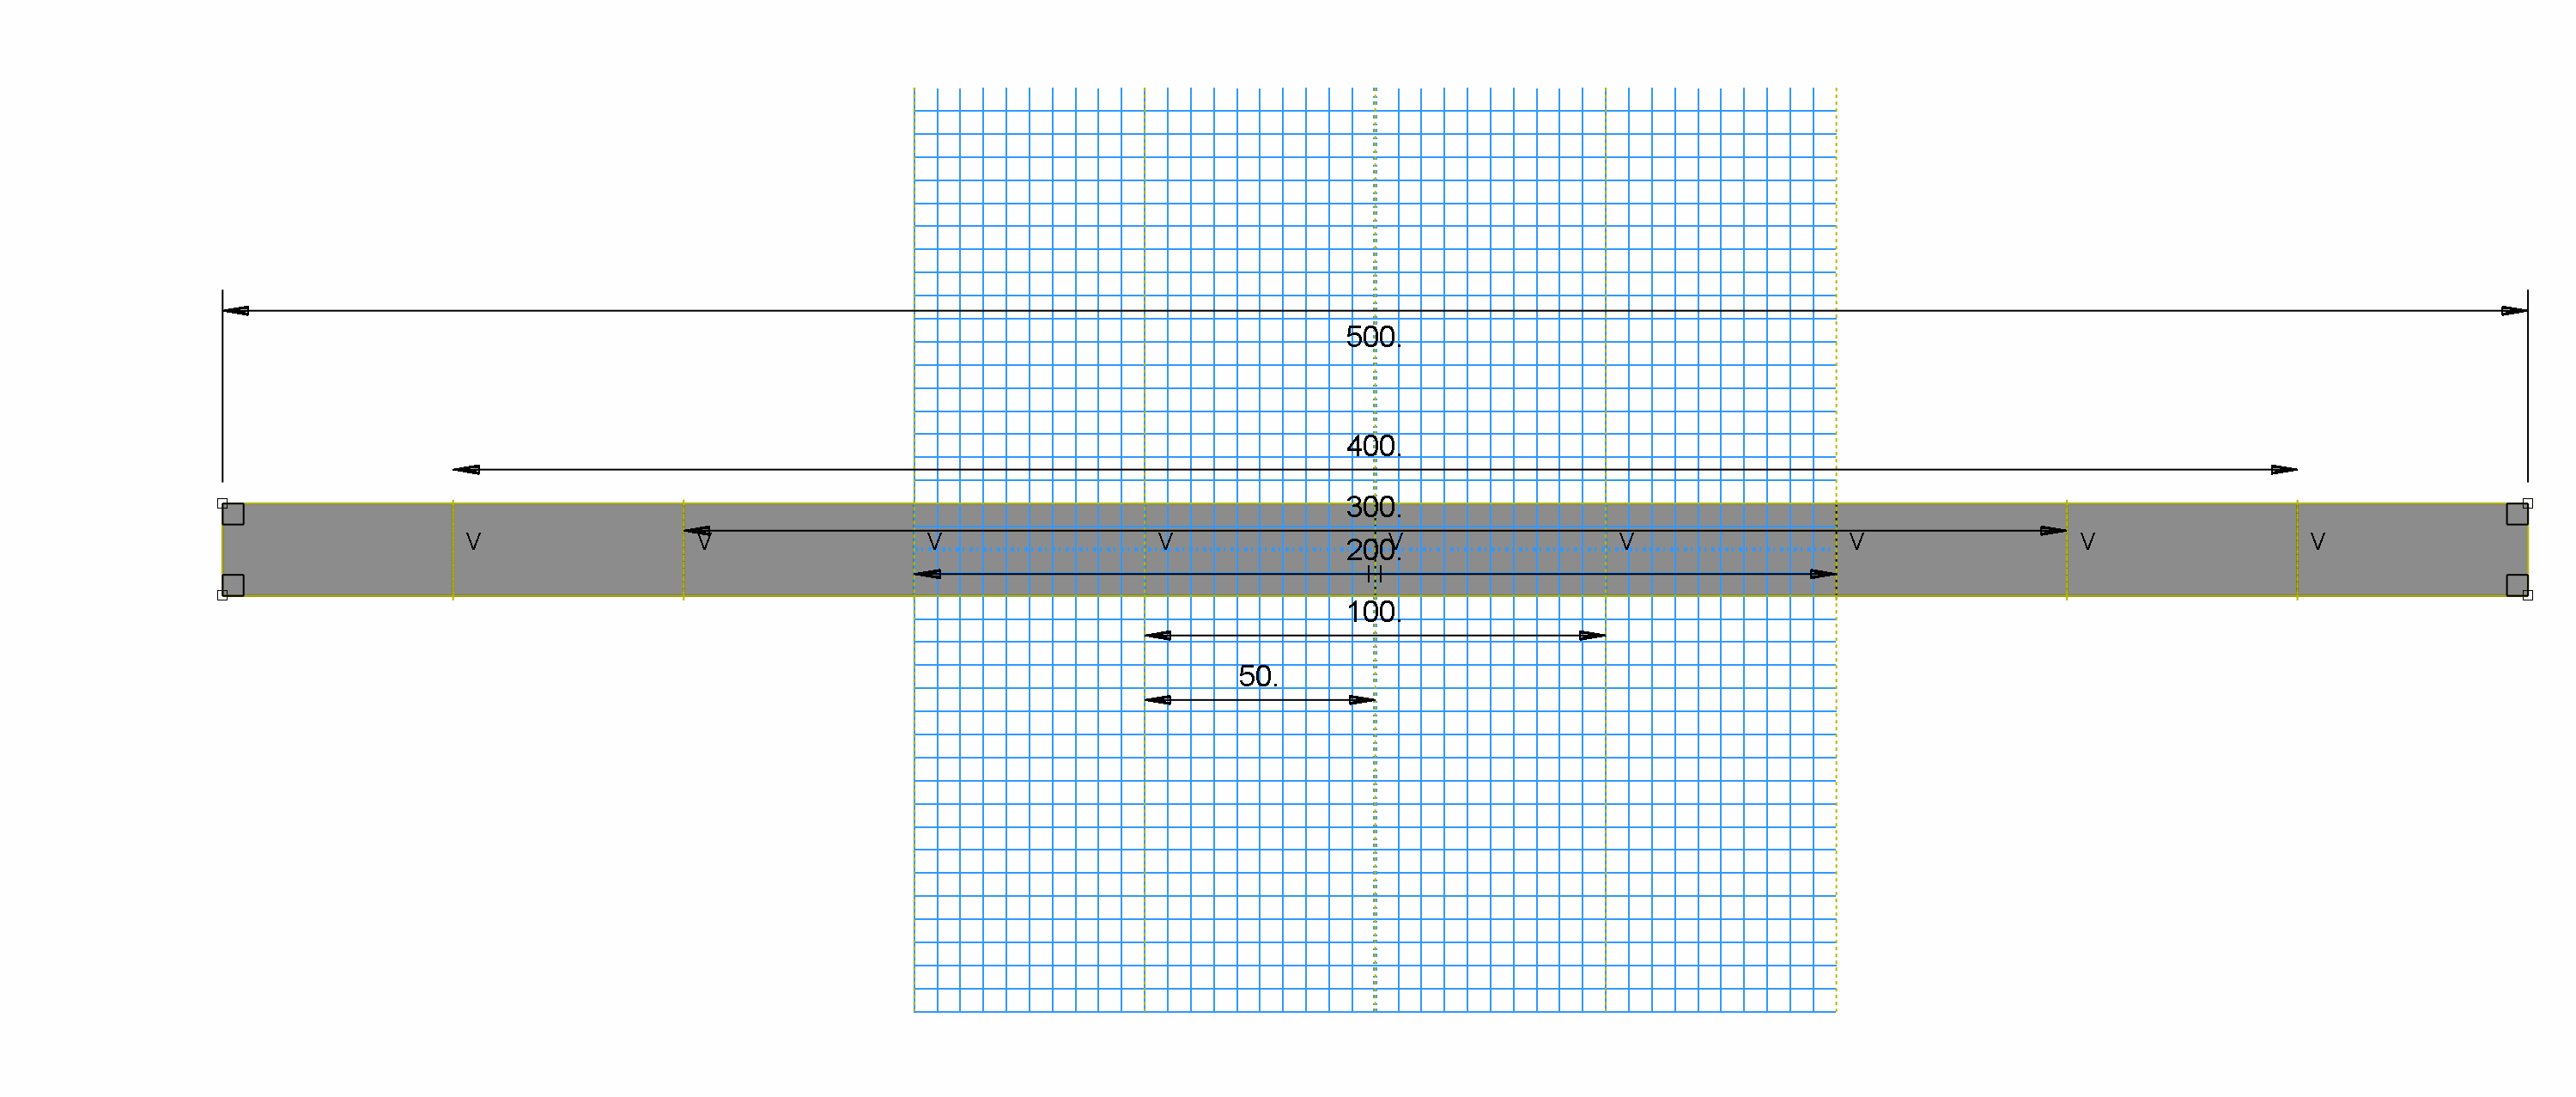
\includegraphics[width=0.6\textwidth]{03.png}
\end{center}

\textbf{河堤}:

河堤为50×50×20的立方体,如图1所示,变长为20的一边与桥面相铰接,另外在距离底面20处与支撑梁相铰接。(铰接指对应结点平动自由度相同,转动自由度自由)

采用实体单元建模。

\begin{center}
\begin{tabular}{ll}
材料&:Granite\\
弹性模量&:60e9\\
泊松比&:0.27\\
密度&:2770\\
\end{tabular}
\end{center}

\textbf{支撑梁}:

支撑梁共有两组,分别位于桥面两侧下方,其结构左右对称,如图4所示。支撑梁上部每个结点与桥面相铰接,两组共计2×9=18个结点。两端结点与河堤相铰接,共计2×2=4个结点。

采用梁单元建模,梁截面为正方形筒,边长为2,厚度为0.1。

\begin{center}
\begin{tabular}{ll}
材料&:Aluminum\\
弹性模量&:70e9\\
泊松比&:0.346\\
密度&:2710\\
\end{tabular}
\end{center}
\begin{center}
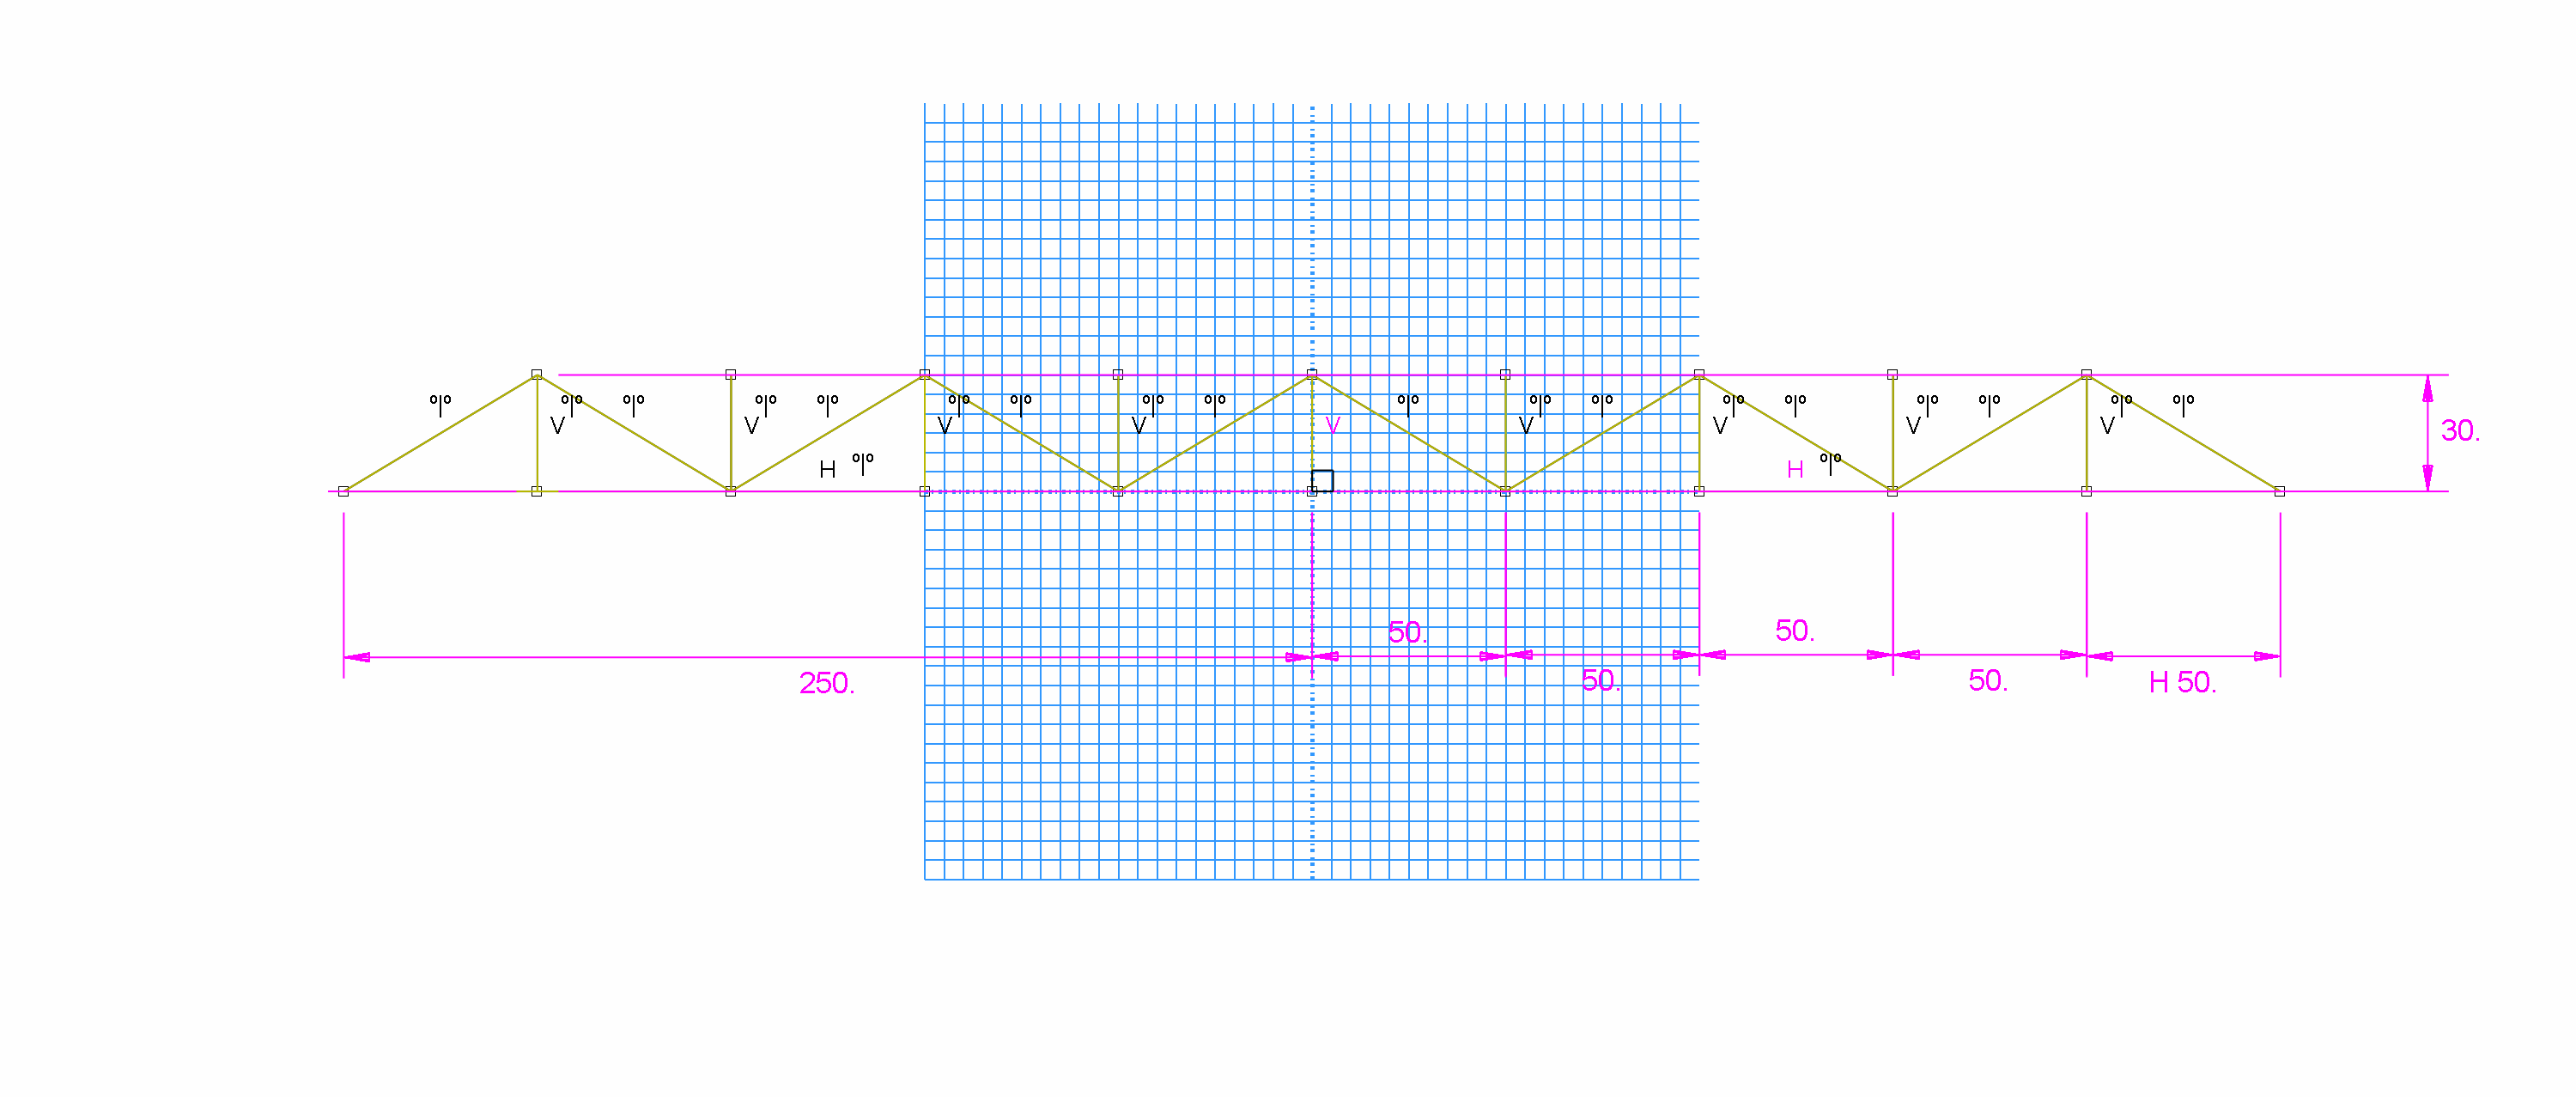
\includegraphics[width=0.6\textwidth]{04.png}
\end{center}

\textbf{钢缆}:

连接桥面与桥墩,共计2×2×5=20根。每根截面积为0.25。

采用杆单元建模

\begin{center}
\begin{tabular}{ll}
材料&:Steel\\
弹性模量&:117e9\\
泊松比&:0.266\\
密度&:7860\\
\end{tabular}
\end{center}

\subsection{Abaqus结果}
\begin{center}
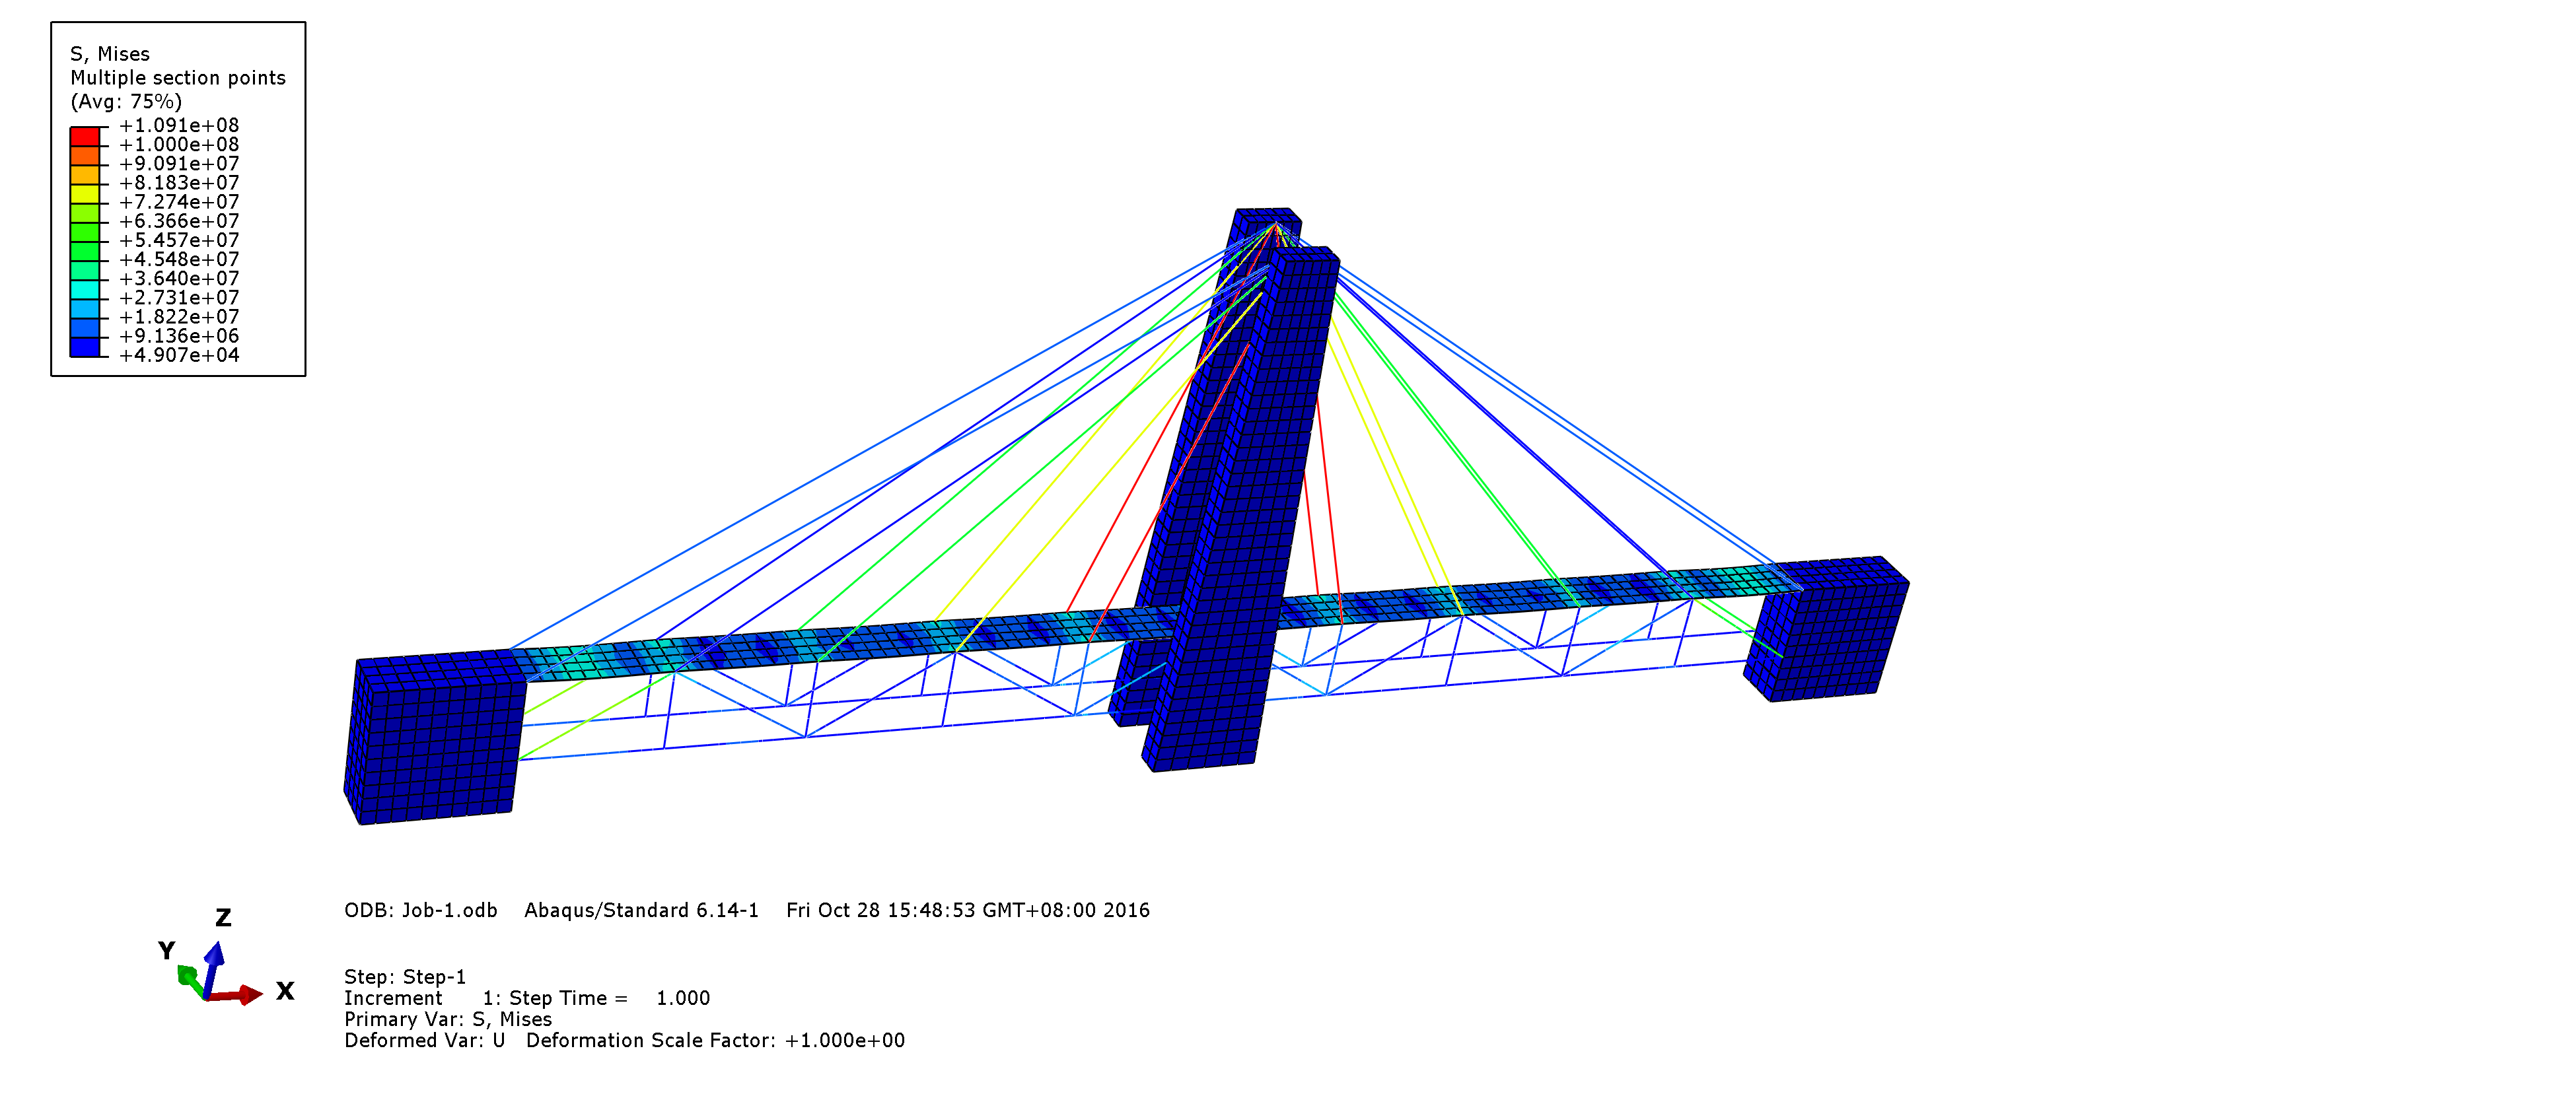
\includegraphics[width=0.6\textwidth]{05.png}
\end{center}


%-------------------------这里是各个部分的描述-------------------------------------
%----------------------------------------------------------------------------------
\section{桥梁功能实现方案}
\subsection{前处理}

%-----------------------------------------------------SPR----------------------------------------------%
\subsection{SPR}

采用SPR方法进行节点应力恢复。对于一个内部节点,若与8个8H单元相连,则有$n=8\times8=64$个高斯点用于应力恢复;对于一个边界面上的节点,则与4个单元相连,有32个高斯点用于应力恢复;同理,对于边界棱上的节点有16个,边界顶点上的节点有8个高斯点。为防止过拟合,对于边界面上的节点和内部节点采用完备二阶多项式进行最小二乘逼近,对于边界棱和边界顶点上的节点采用完备一阶多项式进行最小二乘逼近。以三维单元为例:
\begin{itemize}
\item 对二阶逼近:


\[
\boldsymbol{A}=\begin{bmatrix}1 & x_{1} & y_{1} & z_{1} & x_{1}y_{1} & y_{1}z_{1} & z_{1}x_{1}\\
1 & x_{2} & y_{2} & z_{2} & x_{2}y_{2} & y_{2}z_{2} & z_{2}x_{2}\\
\vdots & \vdots & \vdots & \vdots & \vdots & \vdots & \vdots\\
1 & x_{n} & y_{n} & z_{n} & x_{n}y_{n} & y_{n}z_{n} & z_{n}x_{n}
\end{bmatrix},\ \boldsymbol{X}=\begin{bmatrix}1 & x & y & z & xy & yz & zx\end{bmatrix}
\]



\[
\boldsymbol{C}_{ij}=\begin{bmatrix}c_{0} & c_{1} & c_{2} & c_{3} & c_{4} & c_{5} & c_{6}\end{bmatrix}^{T},\ \boldsymbol{S}_{ij}=\begin{bmatrix}\sigma_{ij}^{(1)} & \sigma_{ij}^{(2)} & \cdots & \sigma_{ij}^{(n)}\end{bmatrix}^{T}
\]



最小二乘逼近为解系数矩阵$\boldsymbol{C}_{ij}$,使得:$\boldsymbol{AC}_{ij}=\boldsymbol{S}_{ij},\ \text{即}\boldsymbol{A}^{T}\boldsymbol{AC}_{ij}=\boldsymbol{A}^{T}\boldsymbol{S}_{ij}$。最后解$\boldsymbol{X}^{(k)}\boldsymbol{C}_{ij}=S_{ij}^{(k)}$为第$k$个节点上的应力。

\item 对一阶逼近:


同理,但只取$1,\ x,\ y,\ z$的项使用。

\item 当连接到一个节点的所有单元具有的高斯点都不足以满足系数要求,或单元采用的为直接刚度法时,转而采用节点平均法恢复应力。这种情况常见于梁、杆、3T单元等。
\item 之前尝试过采用完备二阶多项式进行逼近,然而基本上都会出现过拟合现象。于是从逼近函数里删去平方项,得到的结果相对理想。
\item 算法分析

为得到每个节点对应的Patch,构建节点关系矩阵NodeRelationFlag,为NUMNP行矩阵,列数由单元类型以一般情况下够用来决定。对组内所有单元的连接矩阵作循环,除最后两列外,之前列按顺序存储循环得到的该节点连接的单元编号。倒数第二列指示该节点共连接的单元数,最后一列指示哪个单元的1号节点对应本节点,用于提取节点坐标。之后为按节点循环,得到所连接的单元的高斯点坐标及应力情况,对其按之前所述的方法进行最小二乘逼近,得到系数矩阵。最后根据系数矩阵和本节点的坐标得到本节点的应力情况。

\item 本程序对每一个单元组都采用这种思路进行节点应力恢复,并且按单元组顺序将包含节点的各应力分量输出至.OUT文件中
\end{itemize}

%---------------------------------------------------后处理--------------------------------------------------%
\subsection{后处理}
本程序后处理采用ParaView完成,在程序内包含输出为VTK文件的子程序VTKgenerate

在IND=0阶段,对VTK文件进行初始化,按VTK要求的格式写入文件头和各节点坐标。

在程序执行过程中,会将需要后处理而且要从内存中清除的数据写入3个临时文件中。分别为:

\begin{itemize}
\item $VTK.tmp$:存储位移和应力恢复信息,在WRITED(位移)和PostProcessor(应力)子程序处写入;
\item $VTKNode.tmp$:存储连接矩阵信息,在PostProcessor子程序处写入;
\item $VTKElTyp.tmp$:存储单元类型信息,在ElCal子程序处写入。
\end{itemize}

最后在IND=3阶段读取临时文件中的信息,按顺序整合为单一vtk格式的输出文件。网格形式为UNSTRUCTURED GRID,格式为ASCII,所记录的数据类型为double,包含三个场量:位移场、应力场和Von Mises应力场。以下为通过ParaView渲染生成的桥梁变形及应力分布及局部细节(变形放大倍率100,着色为Von Mises应力):
\begin{center}
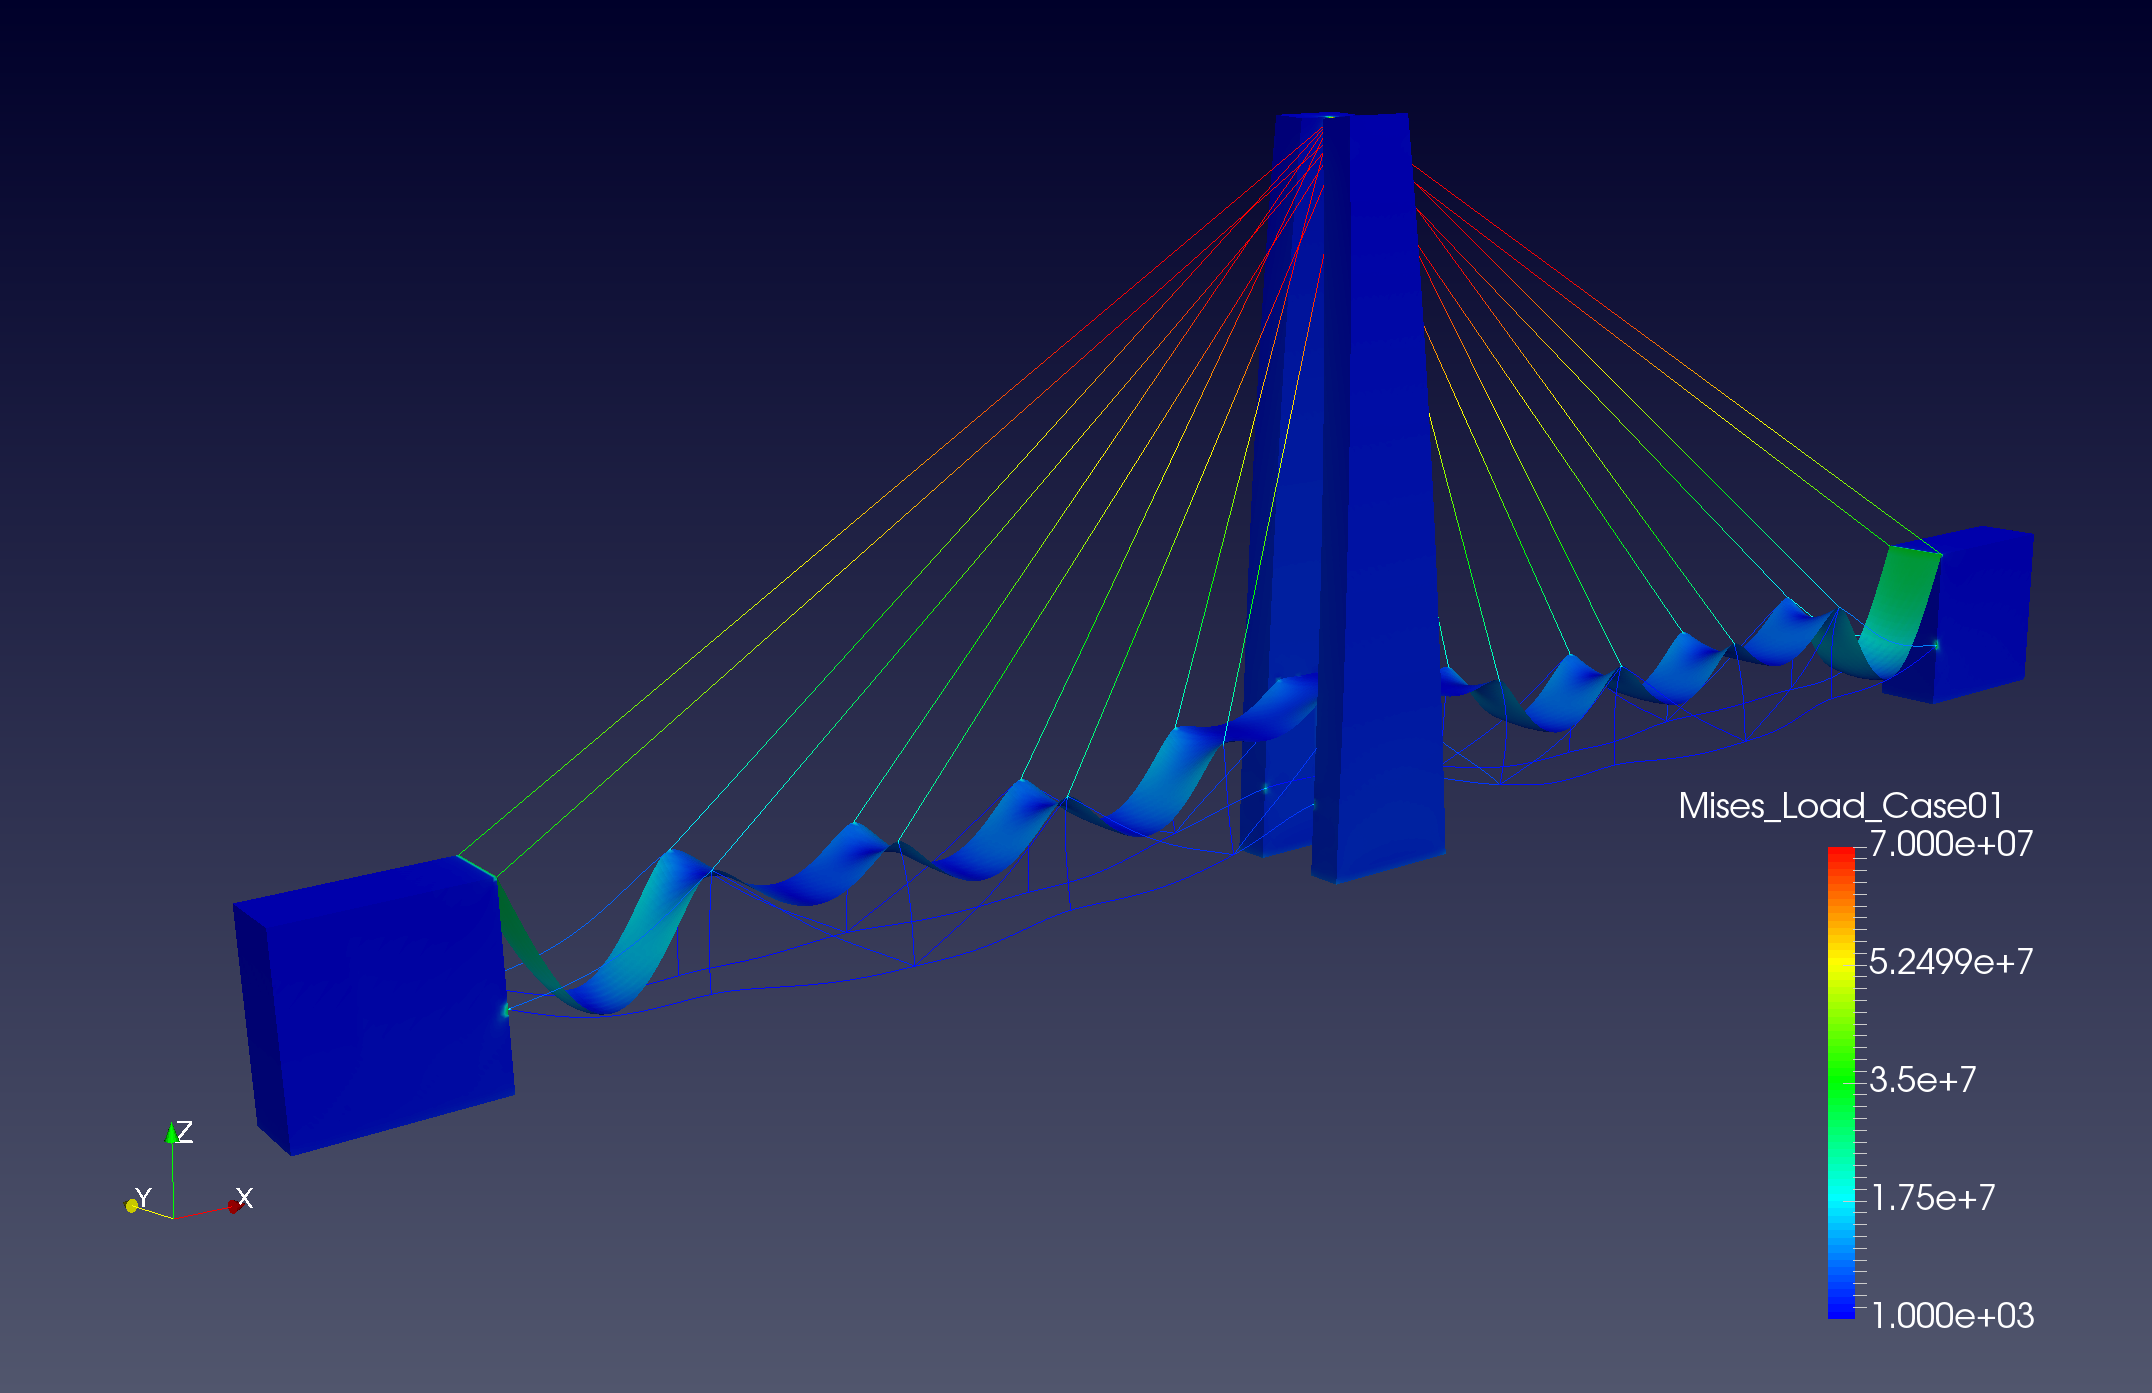
\includegraphics[width=0.8\textwidth]{Bridge-3.png}

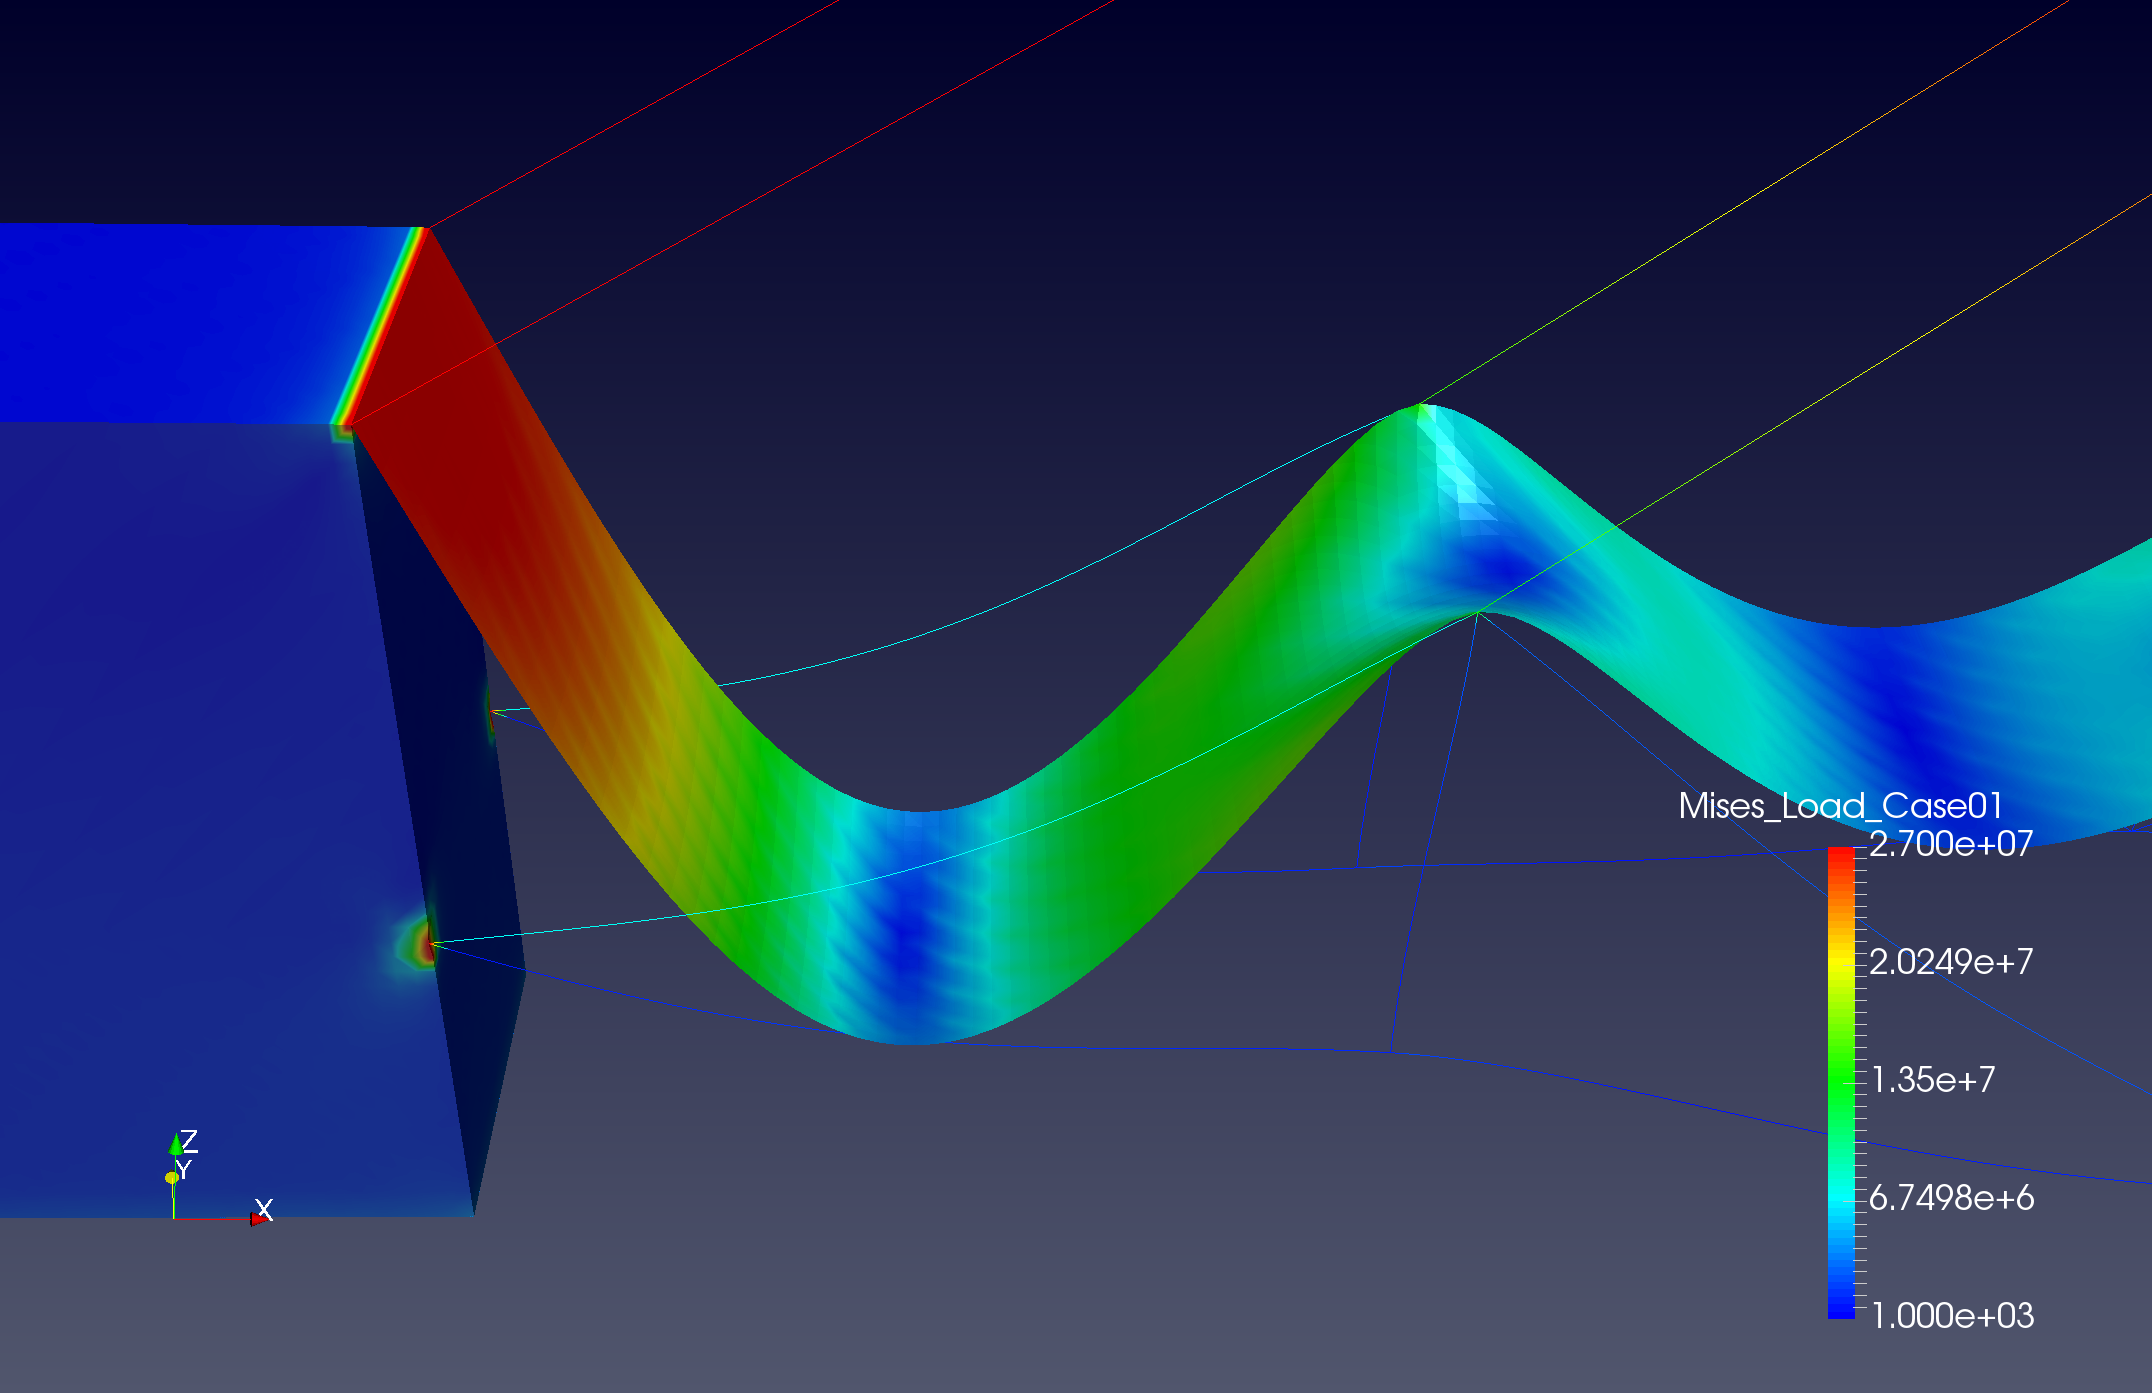
\includegraphics[width=0.8\textwidth]{Bridge-3-part.png}
\end{center}
%-------------------------------------------------------8H--------------------------------------------------%
\subsection{8H}

\begin{itemize}
\item 算法分析

给出一个8H单元,其节点坐标矩阵为$\boldsymbol{X}=\begin{bmatrix}x_{1} & y_{1} & z_{1}\\
x_{2} & y_{2} & z_{2}\\
\vdots & \vdots & \vdots\\
x_{8} & y_{8} & z_{8}
\end{bmatrix}$,每条边的方向上采用2点高斯积分,共8个高斯点,并采用三线性函数作为形函数。作前处理时,将坐标变换到$\xi,\ \eta,\ \zeta$下求形函数的梯度,再对8个高斯点作加权求和,得到单元刚度阵:


\[
N_{i}=\frac{1}{8}(1+\xi_{i}\xi)(1+\eta_{i}\eta)(1+\zeta_{i}\zeta),\ i=1,2,...,8
\]
\[
\boldsymbol{N}=\begin{bmatrix}\boldsymbol{N}_{1} & \boldsymbol{N}_{2} & \boldsymbol{N}_{3} & \boldsymbol{N}_{4} & \boldsymbol{N}_{5} & \boldsymbol{N}_{6} & \boldsymbol{N}_{7} & \boldsymbol{N}_{8}\end{bmatrix},\ \boldsymbol{N}_{i}=N_{i}\begin{bmatrix}1\\
 & 1\\
 &  & 1
\end{bmatrix}
\]
\[
GN=\begin{bmatrix}\frac{\partial N_{1}}{\partial\xi} & \frac{\partial N_{2}}{\partial\xi} & \cdots & \frac{\partial N_{8}}{\partial\xi}\\
\frac{\partial N_{1}}{\partial\eta} & \frac{\partial N_{2}}{\partial\eta} & \cdots & \frac{\partial N_{8}}{\partial\eta}\\
\frac{\partial N_{1}}{\partial\zeta} & \frac{\partial N_{2}}{\partial\zeta} & \cdots & \frac{\partial N_{8}}{\partial\zeta}
\end{bmatrix}
\]



\[
\boldsymbol{B}=\nabla_{s}\boldsymbol{N}=\begin{bmatrix}\boldsymbol{B}_{1} & \boldsymbol{B}_{2} & \boldsymbol{B}_{3} & \boldsymbol{B}_{4} & \boldsymbol{B}_{5} & \boldsymbol{B}_{6} & \boldsymbol{B}_{7} & \boldsymbol{B}_{8}\end{bmatrix},\ \boldsymbol{B}_{i}=\begin{bmatrix}B_{ix} & 0 & 0\\
0 & B_{iy} & 0\\
0 & 0 & B_{iz}\\
B_{iy} & B_{ix} & 0\\
0 & B_{iz} & B_{iy}\\
B_{iz} & 0 & B_{ix}
\end{bmatrix},\ i=1,2,...,8
\]



$\boldsymbol{B}$矩阵的各量由单元Jacobian矩阵和形函数对各坐标的导数得到:


\[
\boldsymbol{J}^{-1}\cdot GN=\begin{bmatrix}B_{1x} & B_{2x} & \cdots & B_{8x}\\
B_{1y} & B_{2y} & \cdots & B_{8y}\\
B_{1z} & B_{2z} & \cdots & B_{8z}
\end{bmatrix},\ \boldsymbol{J}=GN\cdot\boldsymbol{X}^{T}
\]



$\boldsymbol{D}$矩阵由本构关系得到,在此认为材料是各向同性的:


\[
\sigma_{ij}=2G\varepsilon_{ij}+\lambda\varepsilon_{kk}\delta_{ij}
\]
$\Rightarrow\boldsymbol{D}=\begin{bmatrix}2G+\lambda & \lambda & \lambda\\
\lambda & 2G+\lambda & \lambda\\
\lambda & \lambda & 2G+\lambda\\
 &  &  & 2G\\
 &  &  &  & 2G\\
 &  &  &  &  & 2G
\end{bmatrix},\ \text{s.t. }\boldsymbol{\sigma}=\boldsymbol{D\varepsilon},\ \text{where }\boldsymbol{\varepsilon}=\begin{bmatrix}\varepsilon_{x}\\
\varepsilon_{y}\\
\varepsilon_{z}\\
\varepsilon_{xy}\\
\varepsilon_{yz}\\
\varepsilon_{zx}
\end{bmatrix},\ \boldsymbol{\sigma}=\begin{bmatrix}\sigma_{x}\\
\sigma_{y}\\
\sigma_{z}\\
\tau_{xy}\\
\tau_{yz}\\
\tau_{zx}
\end{bmatrix}$.


\[
\boldsymbol{K}^{e}=\sum_{i=1}^{2}\sum_{j=1}^{2}\sum_{k=1}^{2}w_{i}w_{j}w_{k}\boldsymbol{B}^{T}(\xi_{i},\eta_{j},\zeta_{k})\boldsymbol{DB}(\xi_{i},\eta_{j},\zeta_{k})
\]



生成单元刚度阵通过Location Matrix进行组装,得到全局的刚度阵,再解$\boldsymbol{Kd=f}$.


\item 算法实现


位移计算部分按照变换将坐标变换到$[-1,1]\times[-1,1]\times[-1,1]$后即可得到形函数和各导数。取得高斯点位置,代入$\boldsymbol{D}$矩阵即可以产生单元刚度阵,调用COLHT和ADDBAN生成总刚度矩阵并求解。


SPR部分,在前处理时保存单元连接矩阵到临时文件中,在后处理中调取,计算每个节点连接的单元数量和编号,以及用于恢复节点位置的信息,生成为NodeRelationFlag数组。对每个节点,根据该数组选取逼近的阶次,计算$\boldsymbol{A}\text{、}\boldsymbol{S}$矩阵,并传入最小二乘子程序LeastSquare中,得到系数数组,并代入节点位置信息,得到恢复的节点应力。

\item 算法测试


Patch Test 选取了7单元模型和8单元模型进行测试,测试形状为单位立方体,$E=1000,\ \nu=0.25$,通过内部确定1个或8个点来将其分划为8个或7个单元。施加线性位移场:


\[
u_{x}=0.001x,\ u_{y}=0.002y,\ u_{z}=0.003z
\]



得到各点需要施加的外力,并采用最少的边界条件对单元进行测试。测试结果如 data/8H 中各输入输出文件所示。


测试结果表明,对于线性场,输出误差在机器$\varepsilon$量级,单元设计能精确重构线性位移场,为一阶收敛的。


对SPR的测试,其输出结果误差也在机器$\varepsilon$量级,因而从算法设计的角度来说是合理的。




\end{itemize}


\subsection{Beam}
\subsubsection{Basic principles}
\paragraph{}
For a beam element, the equation for a single beam element is quite simple, for the reason that the calculation of the element stiffness matrix doesn't require numerical integral.It can be done manually.
The stiffness matrix for a beam element is as follow.
\begin{center}
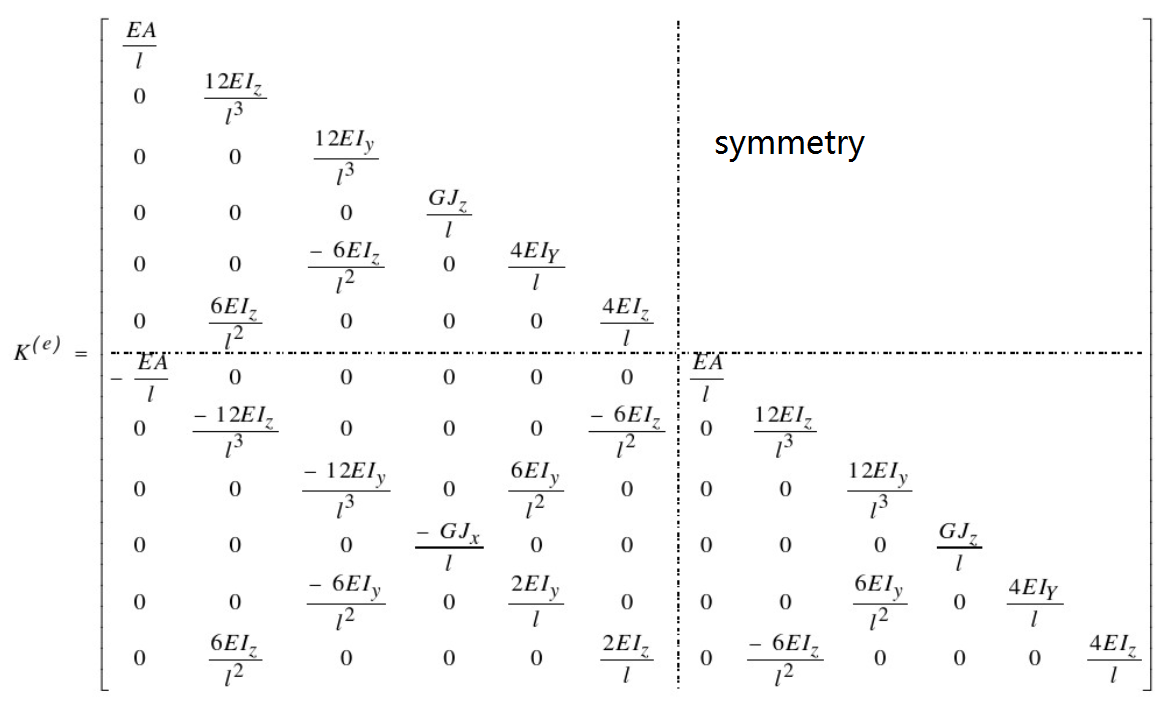
\includegraphics[width=1.0\textwidth]{beam1.png}
\end{center}
\begin{center}
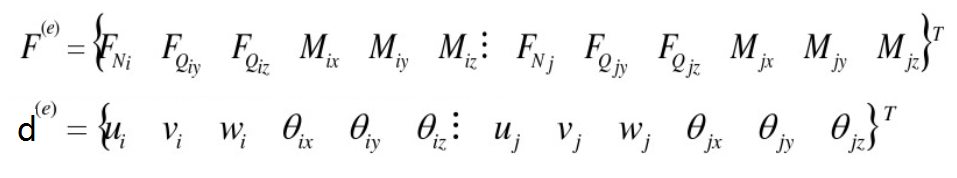
\includegraphics[width=1.0\textwidth]{beam2.png}
\end{center}
In all, we can get the equation for the element itself.
\begin{equation}
{\bf K^{(e)}d^{(e)}=F^{(e)}}
\end{equation}
The process of assembly and solution of the linear equation is just the same as the former elements.
\paragraph{ATTENTION} The stiffness matrix for beams point to arbitrary directions needs the translation matrix to do the coordinates translation.
\begin{equation}
{\bf K^{(e)\prime}=T^{T}K^{(e)}T}
\end{equation}
\subsubsection{Programming procedures}
\paragraph{}
The most difficult part for the programming is the generation of the ID array without interfering with other elements. The structure of the STAP90 program is very terrible for this kind of modification, given the reason that the original program read the element controlling messages after the nodes, making it complex for the dealt for nodes. The only choice left for me is whether changing the whole blueprint for the entire STAP 90 program or just writing the individual input or output subroutine for  the beam. In terms of the deadline requirements, I choose the lateral,leaving the former mission to the following weeks. As you can see in the source files, the input and output subroutine for the beam is in the 'BEAM.f90'.
\subsubsection{Input file format}
\paragraph{}For controlling messages of nodals:
\begin{center}
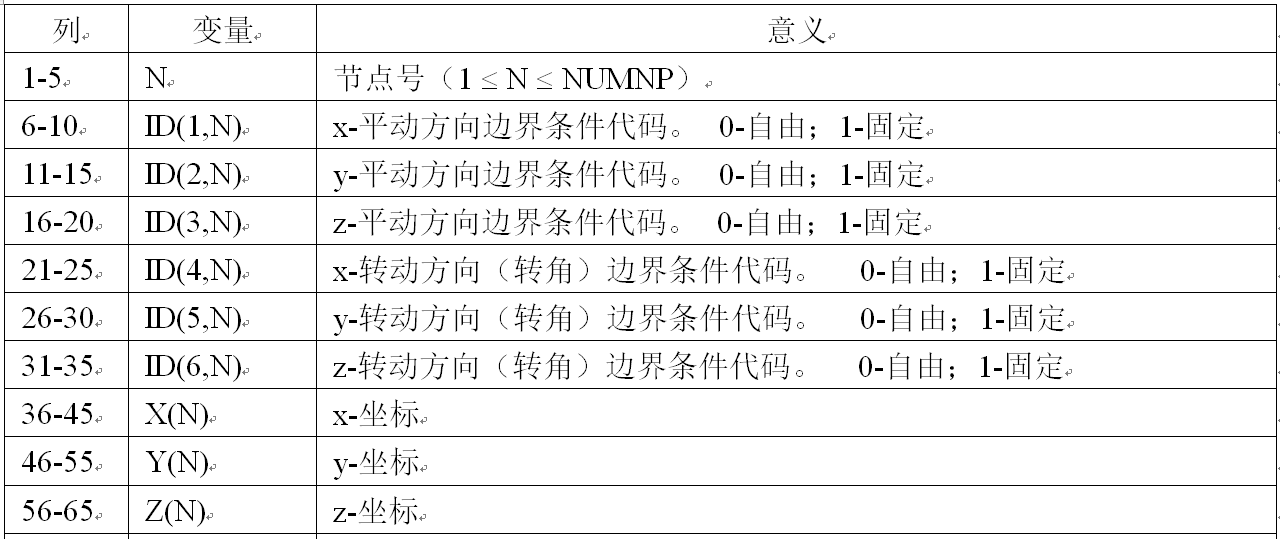
\includegraphics[width=1.0\textwidth]{beam3.png}
\end{center}
\paragraph{}For information about the loads:
\begin{center}
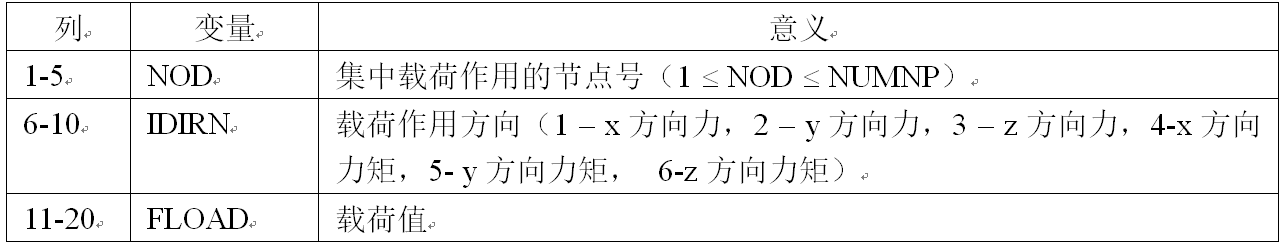
\includegraphics[width=1.0\textwidth]{beam4.png}
\end{center}
\paragraph{}For information about the materials:
\begin{center}
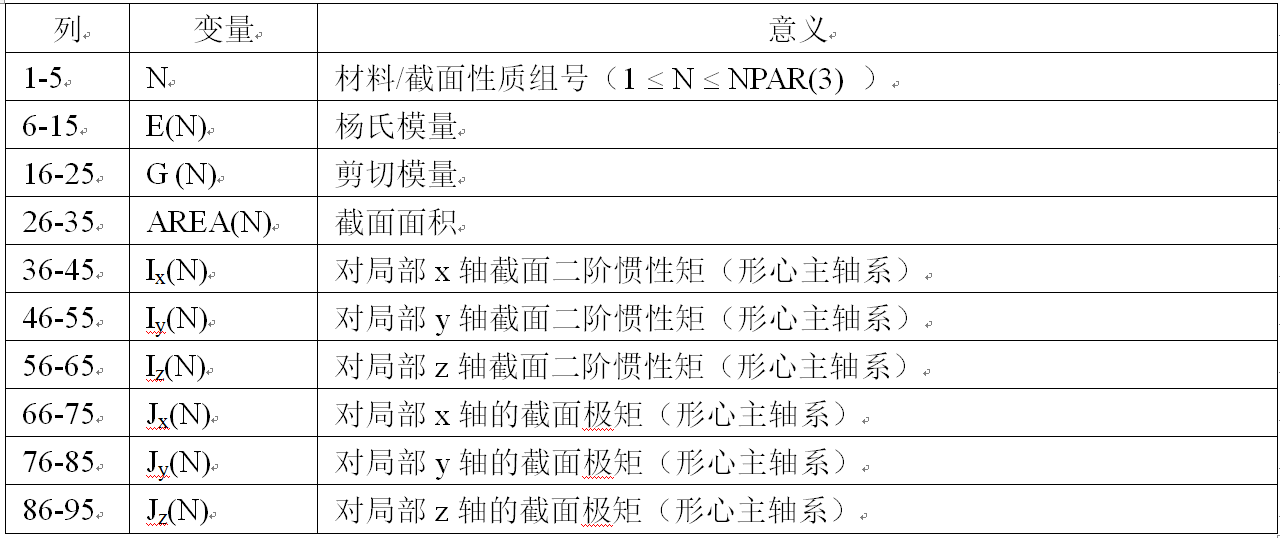
\includegraphics[width=1.0\textwidth]{beam5.png}
\end{center}
\paragraph{}For information about the element connectivity:
\begin{center}
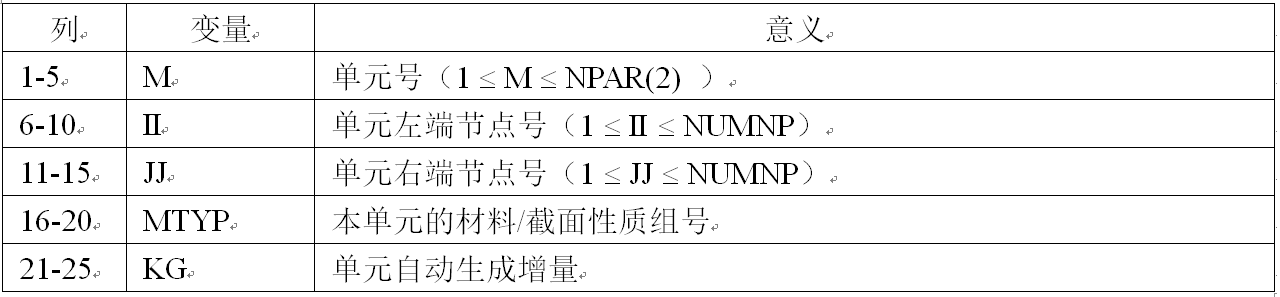
\includegraphics[width=1.0\textwidth]{beam6.png}
\end{center}
\subsubsection{The rate of convergence}
For the beam, the FEM guarantees the continuity and the completeness. The completeness will be verified in the patchtest.For continuity, the method for the approximation of the function is 3-order Hermite interpolation, maintaining the continuity for both the displacement and the angle.It is obvious that the FEM will give the exact answer at nodes if we give concentration forces or momentum at the nodes.For the distribution forces, the FEM will not give the exact results. The reason for this is that the order of the moment is at least 2 for the distribution forces. The results will be better and will converge to the exact solution with the mesh refined to infinite decimal.The convergence rate for the displacement is at the order of 2, while the rate for the energy norm is at the order of 1.
\subsubsection{Patchtest and the results}
I use an example for the patchtest.The situation of the load and the structure is as follow.
\begin{center}
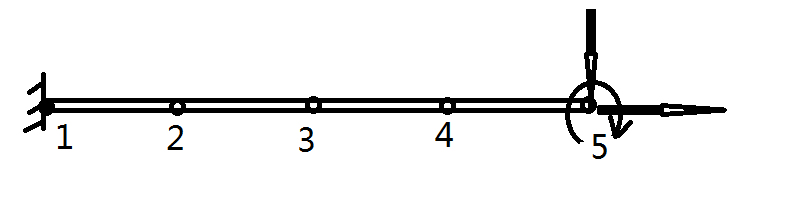
\includegraphics[width=1.0\textwidth]{beam7.png}
\end{center}
The input files and the results for the patchtest in the folder for the beam.
\subsection{Shell}

\subsection{半带宽优化}

\subsection{稀疏存储求解器}

%-------------------------这里是其他单元的描述-------------------------------------
%----------------------------------------------------------------------------------
\section{其他单元}
\subsection{3T}

\subsection{4Q}

\subsection{6T}

\subsection{8Q}

\subsection{9Q}

\subsection{4T}

\subsection{铁木辛柯梁}

\subsection{Plate}

\subsection{无限单元}

\subsection{超级单元}

\subsection{过渡单元}

%-------------------------这里是其他功能的描述-------------------------------------
%----------------------------------------------------------------------------------
\section{高级功能}
\subsection{弹塑性杆分析}





\subsubsection{基本原理}
\paragraph{}
弹塑性杆是一种最简单的材料非线性问题。在这个功能中,我使用切线刚度法来进行求解。我把杆的塑性问题简化成弹性段和塑形段,其中每段近似成线性函数,并使用相应的弹性模量和塑形模量来表示两端线段的斜率。切线刚度法的基本思想就是:假使载荷为$P_A$时,相应的位移为$u_A$,切线刚度为$K_A$,那么对于下一次载荷增量产生的位移是,
$$K_A\triangle u_{AB}=\triangle f_{AB}$$
$$u_B=u_A+\triangle u_{AB}$$
我们在使用切线刚度法进行计算时,都是从A点的应力状态出发,最后就得到载荷B情况下的各项参数,本方法的特点是,对于一次载荷分量,只需要求解一次即可。
示意图如下。
\begin{center}
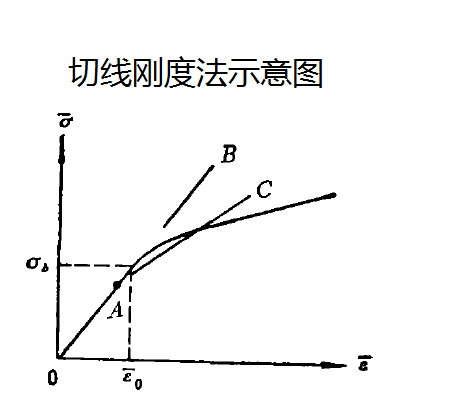
\includegraphics[width=0.6\textwidth]{plastic7.png}
\end{center}
该方法参考了1982年固体力学学报《弹塑性有限元一些解法的比较》,由中科院力学研究所吴永礼先生著。
\subsubsection{编程思路}
\paragraph{}
首先进行弹性试探步的计算,确定是否需要进行弹塑性分析。若进行弹塑性分析,则使用切线刚度法求解。首先把载荷分成很多细份,从零开始逐渐加载。使用切线刚度,算出每一步的位移增量和应力增量,计算每步加载后的位移和应力,同时判断是否有杆进入弹塑性,若有弹塑性变化,则下一次组装刚度阵时要更新。这种增量步的方法把一个非线性的问题线性化,实质上是微分的思路——把复杂的函数简单化,理论上,这种求解方式可以进行任何材料非线性问题的计算。在这个方法中,每一步更新需要前一步的历史位移和应力信息,这些都记录在临时文件里,每一步均更新。
整个程序的流程图如下。
\begin{center}
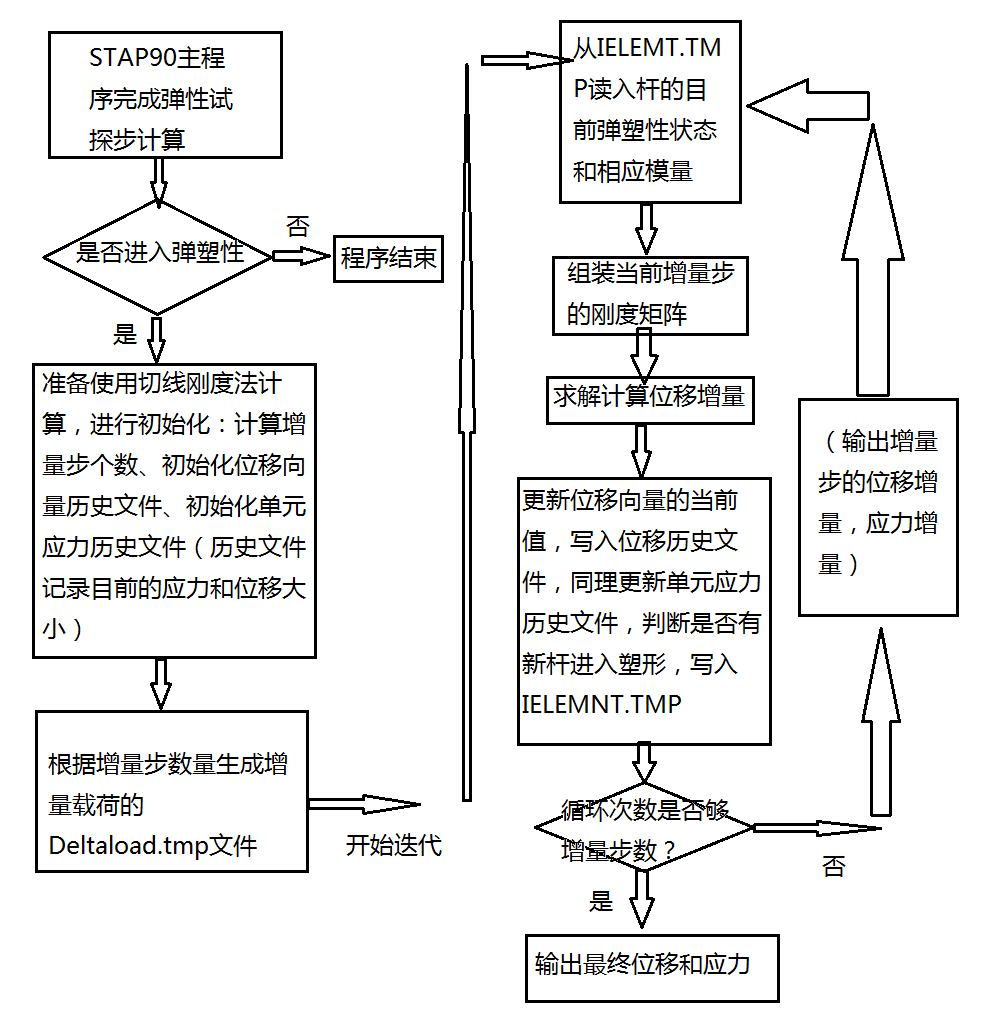
\includegraphics[width=0.9\textwidth]{plastic3.png}
\end{center}
\subsubsection{输入和输出结果}
\paragraph{}
在一根杆上加了100000的力,材料的截面性质如下,各输入和输出如下,结果符合理论值。
\begin{center}
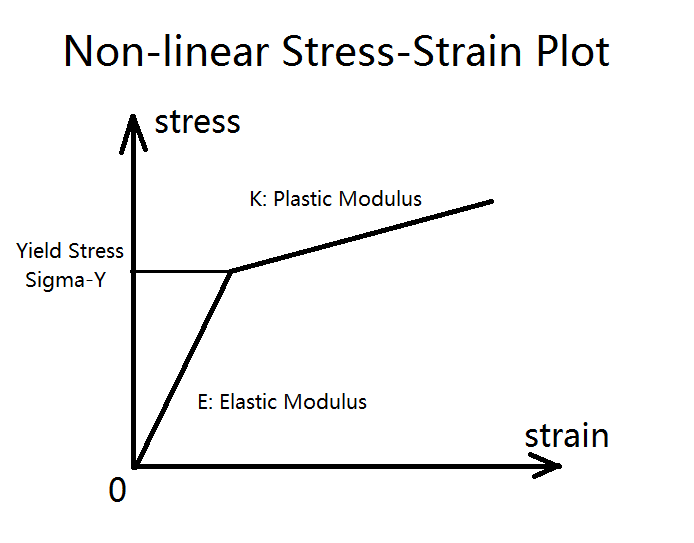
\includegraphics[width=0.5\textwidth]{plastic2.png}
\end{center}
\begin{center}
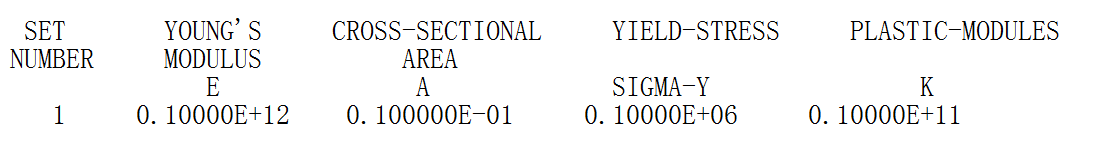
\includegraphics[width=0.8\textwidth]{plastic1.png}
\end{center}
\begin{center}
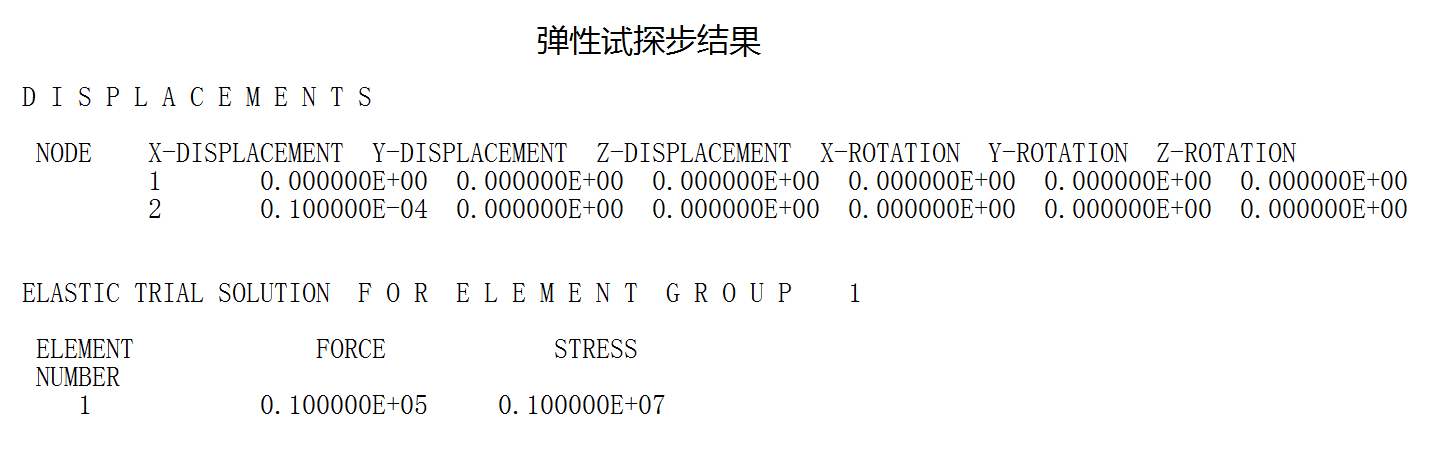
\includegraphics[width=1.0\textwidth]{plastic4.png}
\end{center}
\begin{center}
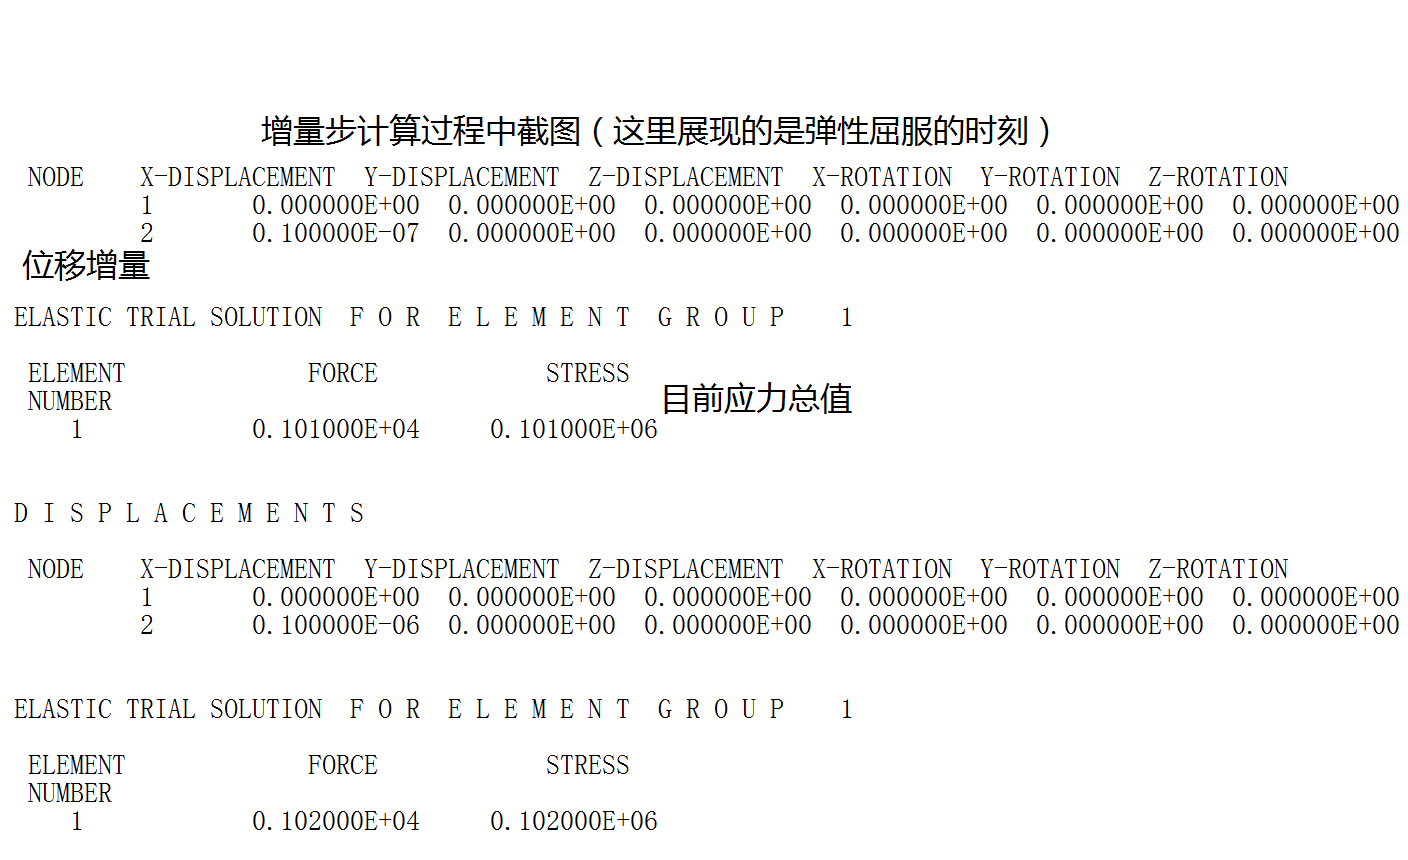
\includegraphics[width=1.0\textwidth]{plastic5.png}
\end{center}
\begin{center}
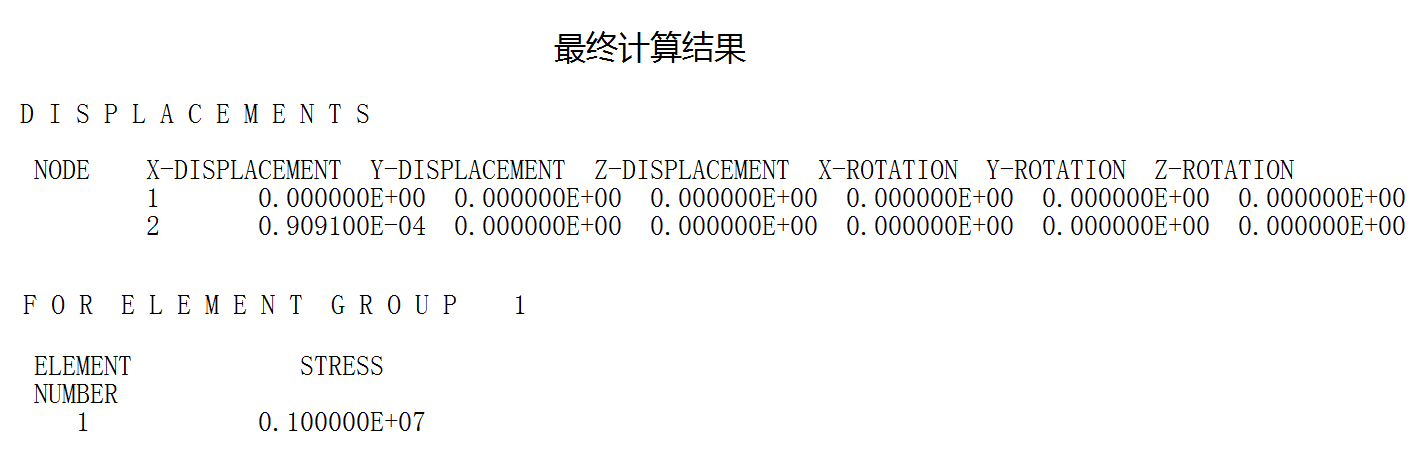
\includegraphics[width=1.0\textwidth]{plastic6.png}
\end{center}
\subsection{模态分析}


\subsection{动力学响应分析}

\end{document}
